\section{Physical Refinement Guarantee}
\label{sec:theorem}

The same-request example in Section~\ref{sec:model} shows why field-wise attenuation alone does not order runtime outputs. \zonecap{} instead separates authorization inclusion from emission inclusion and requires parent realizability at their interface. Fig.~\ref{fig:refinement} summarizes this proof chain and instantiates the resulting reachable-set relation on three exact signed one-dimensional plants.

\begin{figure*}[t]
\centering
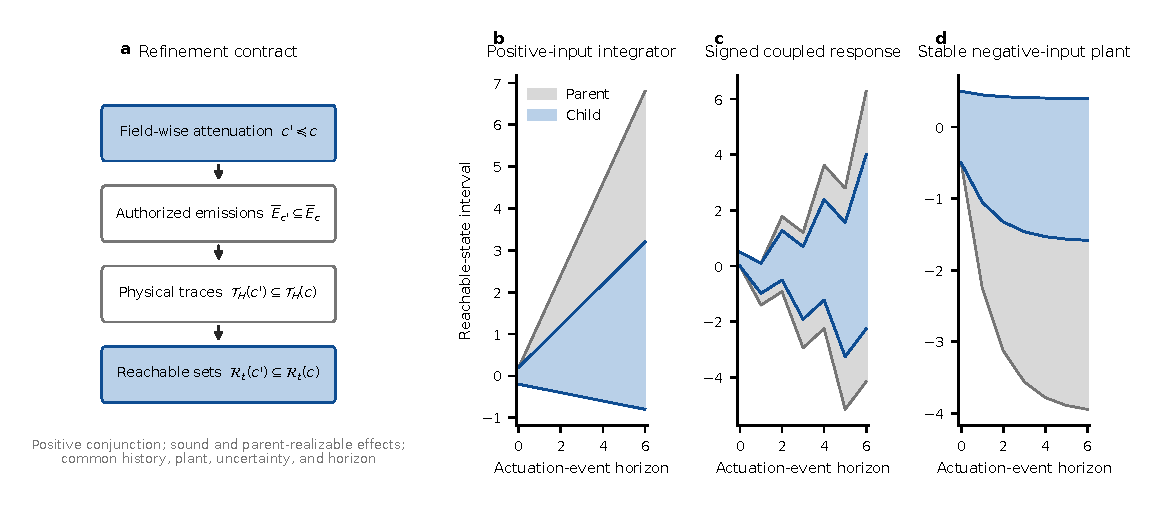
\includegraphics[width=\textwidth]{figures/generated/fig02_refinement_reachability}
\caption{Attenuation-to-reachability refinement and exact instantiations. (a) The proof factors field-wise attenuation through request-abstracted emission and physical-trace inclusion. (b)--(d) Parent and child reachable intervals through actuation-event horizon six for a positive-input integrator, a signed coupled response, and a stable negative-input plant. Grey denotes the parent domain and blue the child domain. The intervals were propagated with seedless exact rational arithmetic; no sampling error bars apply. These panels check executable instances, whereas Theorem~1 establishes the conditional general result.}
\label{fig:refinement}
\end{figure*}

\subsection{Proof Obligations}

The refinement requires six obligations. First, attenuation is the syntactic order in~\eqref{eq:attenuation}, not a definition based on emissions or reachability. Second, positive caveats combine conjunctively; fallback grants and unproved non-monotone conflict combiners are excluded. Third, the child history language refines the parent's, and both evaluate the same physical-history projection. These obligations constrain capability construction.

Three further obligations connect authorization to the plant. Fourth, every emitted rewrite or hold is within the effective capability and parent-realizable; no-command effects contribute no actuation event. Fifth, parent and child use identical $F$, $X_0$, $W$, and horizon. Sixth, reachability is the union over all admitted physical-input and disturbance sequences. It is not a same-request noninterference property, a probability distribution, or a selected controller trajectory.

\subsection{Compiler and Emission Refinement}

\noindent\textbf{Lemma 1 (compiler refinement):} Under obligations 1--3,
\begin{equation}
 c'\preceq c \Longrightarrow
 \Adm_{c'}(\eta)\subseteq\Adm_c(\eta), \quad \forall\eta.
 \label{eq:compiler-refinement}
\end{equation}
Every primitive child domain is a subset of its parent domain. Membership in their positive conjunction therefore implies membership in the parent conjunction. Extending the required event sequence also makes every child-accepted physical history parent-accepted. This argument uses no semantic reachability premise.

\noindent\textbf{Lemma 2 (emission refinement):} Under Lemma~1 and obligation~4,
\begin{equation}
 \overline{E}_{c'}(\eta)\subseteq\overline{E}_c(\eta), \quad \forall\eta.
 \label{eq:emission-refinement}
\end{equation}
Soundness places each ordinary child output in $\Adm_{c'}(\eta)$ and hence in $\Adm_c(\eta)$. Parent realizability supplies a raw parent request that emits the same action. The common hold clause covers a deferred child, while no-output effects add no action to~\eqref{eq:emission}. Authorization membership alone would be insufficient because a parent enforcer could be sound yet unable to produce the child's chosen correction.

\subsection{Trace and Reachable-Set Inclusion}

\noindent\textbf{Theorem 1 (attenuation monotonicity):} Under obligations 1--6, for every finite $H$,
\begin{equation}
 \begin{split}
 c'\preceq c &\Longrightarrow \Tr_H(c')\subseteq\Tr_H(c),\\
 \Tr_H(c')\subseteq\Tr_H(c) &\Longrightarrow
 \Reach_t(c')\subseteq\Reach_t(c),\quad t\leq H.
 \end{split}
 \label{eq:main-theorem}
\end{equation}
The proof is induction on physical transitions. Length-zero traces share $X_0$. Suppose a child trace through $\eta_t$ is also a parent trace. Lemma~2 places its next input in the parent emission relation at the same history. Choosing the same $w_t\in W$ and applying the common $F$ produces the same successor. The extended child trace is therefore a parent trace, and projection onto $x_t$ yields reachable-set inclusion.

For $x_{t+1}=a x_t+b u_t+w_t$ with interval sets, linear images and Minkowski addition preserve inclusion for signed $a$ and $b$, giving an exact one-dimensional corollary. The transition-system proof also covers MIMO and nonlinear plants whenever~\eqref{eq:emission-refinement} holds at every related history. A convex over-approximation alone does not establish this relation. Non-monotone grants, an unauthorized or parent-unrealizable effect, mismatched history or plant semantics, and an unverified fixed-tick idle action are explicit failure conditions rather than implementation details.
